\newcommand{\econtexRoot}{.}
\documentclass{beamer}\usepackage{dcolumn}
% \documentclass[aspectratio=169]{beamer}
\usepackage{verbatim}
\usepackage{cancel}
\usepackage{econtexShortcuts}
\usepackage{wasysym,ifthen,mathrsfs}
\usepackage[english]{babel}
\usepackage{color}
\usepackage[latin1]{inputenc}
\usepackage{booktabs,natbib}
../Switches.tex
\pdfmapfile{+sansmathaccent.map}

%%% Jirka's colors

\definecolor{myRed}{rgb}{0.8,0,0}
\definecolor{jirkasblue}{rgb}{0.2,0.2,0.7}
\definecolor{jirkasred}{rgb}{0.9,0,0}
\definecolor{LightCyan}{rgb}{0.88,1,1}
\definecolor{SlideNavy}{rgb}{0,0,0.54}
\definecolor{StataDarkBlue}{rgb}{0,0,0.835}
\definecolor{Pink}{rgb}{1,0.8,0.8}

\newcolumntype{g}{>{\columncolor{Pink}}d{3}}
\newcommand{\jemph}[1]{{\color{StataDarkBlue}#1}}
\newcommand{\jbemph}[1]{\textbf{\color{SlideNavy}#1}}
\newcommand{\var}{\ensuremath{\text{var}}}

%%%%%%%%%%%%%%%  Beamer setup
%%%%%%%%%%%%%%%%%%%%%%%%%%%%%%%%%%%%%%%%%%%%%%%%%%%%%%%%%%%%%%%%%%%%%%%%%%%%%%%%%%%%%%%%%%%%%%%%%%%%%%%%%%%%%%
\mode<presentation>
{
  \usetheme{Warsaw} % Singapore % Montpellier
  \setbeamercovered{transparent}
}

% if this is on, bullets are shown step by step
%\beamerdefaultoverlayspecification{<+->}

%\setbeamertemplate{navigation symbols}{}  % Take away navigation symbols


%%%%%%%%%%%%%%%  Chris's definitions
%%%%%%%%%%%%%%%%%%%%%%%%%%%%%%%%%%%%%%%%%%%%%%%%%%%%%%%%%%%%%%%%%%%%%%%%%%%%%%%%%%%%%%%%%%%%%%%%%%%%%%%%%%%%%%

\providecommand{\W}{\mathcal{W}}            % Include or exclude aggregate wage in individual problem - to include, should be
\providecommand{\perc}[1]{\widetilde{#1}}

\provideboolean{Depreciation}
\setboolean{Depreciation}{true}
%\setboolean{Depreciation}{false}
\provideboolean{MicroDepr}
\setboolean{MicroDepr}{true}
%\setboolean{Depreciation}{false}
\providecommand{\ifDepr}{\ifthenelse{\boolean{Depreciation}}}
\providecommand{\MicroDepr}{\ifthenelse{\boolean{MicroDepr}}}

\ifDepr{
\providecommand{\RBet}{\mathbf{R}} % Bold  version is between-period rate; \mathcal version is within
\providecommand{\rBet}{\mathbf{r}} % Bold  version is between-period rate; \mathcal version is within
\providecommand{\RIn}{\mathcal{R}}
\providecommand{\rIn}{r}
}{
\providecommand{\RBet}{R} % Bold  version is between-period rate; \mathcal version is within
\providecommand{\rBet}{r} % Bold  version is between-period rate; \mathcal version is within
\providecommand{\RIn}{R}
\providecommand{\rIn}{r}
\providecommand{\rNet}{\mathfrak{r}} % For defining consumption Euler equation
}


\provideboolean{Growth}
\setboolean{Growth}{true}
\setboolean{Growth}{false}
\providecommand{\ifGG}{\ifthenelse{\boolean{Growth}}}  % Switch for whether to include productivity growth in formulae; useful for programming/debugging

\provideboolean{numSwitch}     % Switch that suppresses eqn numbers on slides but not in text
\setboolean{numSwitch}{true}   % Set to true  at beginning of text
%\setboolean{numSwitch}{false} % Set to false at beginning of slides
\providecommand{\ifnumSw}{\ifthenelse{\boolean{numSwitch}}{}{\nonumber}}

\provideboolean{Slides}
\setboolean{Slides}{false}
\providecommand{\ifslides}{\ifthenelse{\boolean{Slides}}}

\provideboolean{ZeroProb}
\setboolean{ZeroProb}{false}
\setboolean{ZeroProb}{true}
\providecommand{\ifZero}{\ifthenelse{\boolean{ZeroProb}}}

\provideboolean{DocVersion} % If true, produce an elaborate version of the document that contains all formulae used in the software
\setboolean{DocVersion}{false}
\setboolean{DocVersion}{true}
\providecommand{\ifDoc}{\ifthenelse{\boolean{DocVersion}}}

% ExtraExplain toggles whether to include the explanation for why we can't assume \bar{\ell}=\ell
\provideboolean{ExtraExplain}
\setboolean{ExtraExplain}{true}
\providecommand{\ifExplain}{\ifthenelse{\boolean{ExtraExplain}}}

\provideboolean{ShowStickyE}
\setboolean{ShowStickyE}{true}
\setboolean{ShowStickyE}{false}
\providecommand{\StickyE}{\ifthenelse{\boolean{ShowStickyE}}}

\providecommand{\econtexRoot}{.}
\providecommand{\eq}{\econtexRoot/Equations}

\providecommand{\fm}{frictionless-$\mathbf{m}$ }
\providecommand{\sm}{sticky-$\mathbf{m}$ }

\providecommand{\ParmDir}{\econtexRoot/Calibration/Parameters}
\providecommand{\TablesDir}{\TabsDir}
%\providecommand{\ParmDir}{C:/Jirka/Research/stickyConsumptionUS/Nov26_07/cAndCwithStickyEArchive/Calibration/Parameters}
%\providecommand{\TablesDir}{C:/Jirka/Research/stickyConsumptionUS/Nov26_07/cAndCwithStickyEArchive/Tables}

%%%%%%%%%%%%%%%  Jirka's definitions
%%%%%%%%%%%%%%%%%%%%%%%%%%%%%%%%%%%%%%%%%%%%%%%%%%%%%%%%%%%%%%%%%%%%%%%%%%%%%%%%%%%%%%%%%%%%%%%%%%%%%%%%%%%%%%

%\input EconDocStart
%\input PDFDocStart
\mode<presentation>
{
  \usetheme{Warsaw}
  % or ...

  \setbeamercovered{transparent}
  % or whatever (possibly just delete it)
}
\definecolor{jirkasred}{rgb}{0.9,0,0}
\definecolor{jirkasblue}{rgb}{0.2,0.2,0.7}
\providecommand{\jemph}[1]{{\color{jirkasblue}#1}}
\def\newblock{\hskip .11em plus .33em minus .07em}


\newcolumntype{d}[1]{D{.}{.}{#1}}

\usepackage[latin1]{inputenc}
% or whatever

%%%%%%%%%%%%%%%  Opening slide
%%%%%%%%%%%%%%%%%%%%%%%%%%%%%%%%%%%%%%%%%%%%%%%%%%%%%%%%%%%%%%%%%%%%%%%%%%%%%%%%%%%%%%%%%%%%%%%%%%%%%%%%%%%%%%


\title[Sticky Expectations and Consumption Dynamics]{Sticky Expectations and Consumption Dynamics}

\author[Carroll, Crawley, Slacalek, Tokuoka, White]{Christopher D. Carroll\inst{1} \and Edmund Crawley\inst{2} \and Jiri Slacalek\inst{3} \and Kiichi Tokuoka\inst{4} \and Matthew N. White\inst{5}}

%\institute % (optional, but mostly needed)
%{
%Board of Governors of the Federal Reserve System
%}
% - Use the \inst command only if there are several affiliations.
% - Keep it simple, no one is interested in your street address.
\institute{
  \inst{1} Johns Hopkins and NBER, \texttt{ccarroll@jhu.edu} %\\ \texttt{http://www.econ.jhu.edu/people/ccarroll/}
  \and
  \inst{2} Johns Hopkins,  \texttt{ecrawle2@jhu.edu} %\\ \texttt{http://www.slacalek.com/}
  \and
  \inst{3} European Central Bank,  \texttt{jiri.slacalek@ecb.int} %\\ \texttt{http://www.slacalek.com/}
  \and
  \inst{4} MoF Japan,  \texttt{kiichi.tokuoka@mof.go.jp}
  \and
 \inst{5} University of Delaware,  \texttt{mnwecon@udel.edu}\\
  }
\date{Computing in Economics and Finance, Milan\\[4mm] June 2018 % venue
}

\begin{document}

\newcolumntype{d}[1]{D{.}{.}{#1}}
\def\newblock{\hskip .11em plus .33em minus .07em}

\begin{frame}
  \titlepage
\end{frame}


%%%%%%%%%%%%%%% Other slides
%%%%%%%%%%%%%%%%%%%%%%%%%%%%%%%%%%%%%%%%%%%%%%%%%%%%%%%%%%%%%%%%%%%%%%%%%%%%%%%%%%%%%%%%%%%%%%%%%%%%%%%%%%%%%%

%\section{Consumption: Micro Vs Macro}
%\subsection{Habits?  No!  It's Inattention}
\begin{frame}
  \frametitle{Consumption Dynamics: Macro vs Micro}
%  \jbemph{\large C growth persistent in macro but not micro data}
  \begin{block}{Macro: Representative Agent Models}
      \begin{itemize}
      \item  Theory (With Separable Utility):
        \begin{itemize}
        \item         C responds instantly, completely to shock
          \item Consequences of uncertainty are trivial
        \end{itemize}
%        \item Uncertainty has trivial effects
    \item Evidence: Consumption is too smooth {\scriptsize (Campbell {\&} Deaton, 1989)}
      \item Solution: \jbemph{``Habits'' parameter $\chi^{\text{Macro}}\approx 0.6$--$0.8$}\\
\centerline{       $\Delta \log \mathbf{C}_{t+1} = \varsigma + \chi \Delta \log \mathbf{C}_t +\epsilon $}
      \end{itemize}
    \end{block}

  \begin{block}{Micro: Heterogeneous Agent Models}
    \begin{itemize}
    \item  \jbemph{Uninsurable risk is essential, changes everything}
    \item Var of micro income shocks much larger than of macro shocks:\\
\centerline{    \jemph{var$(\Delta \log \pLevBF) \approx  100\times$var($\Delta \log \PLevBF$)}}
    \item Evidence: \jbemph{``Habits'' parameter $\chi^{\text{Micro}}\approx 0.0$--$0.1$}
    \end{itemize}
  \end{block}

\end{frame}

\begin{frame}
  \frametitle{Persistence of Consumption Growth: Macro vs Micro}

  \begin{itemize}
  \item New paper in EER, \cite*{havranek:metaHabits}\\ ~~~~Meta analysis of 597 estimates of $\chi$
  \item $ \Delta \log \mathbf{C}_{t+1} = \varsigma + \chi \Delta \log \mathbf{C}_t +\epsilon $
  \item  \jemph{$\{\chi^{\text{Macro}},\chi^{\text{Micro}}\} = \{0.6,0.1\}$}
  \begin{figure}
\begin{center}
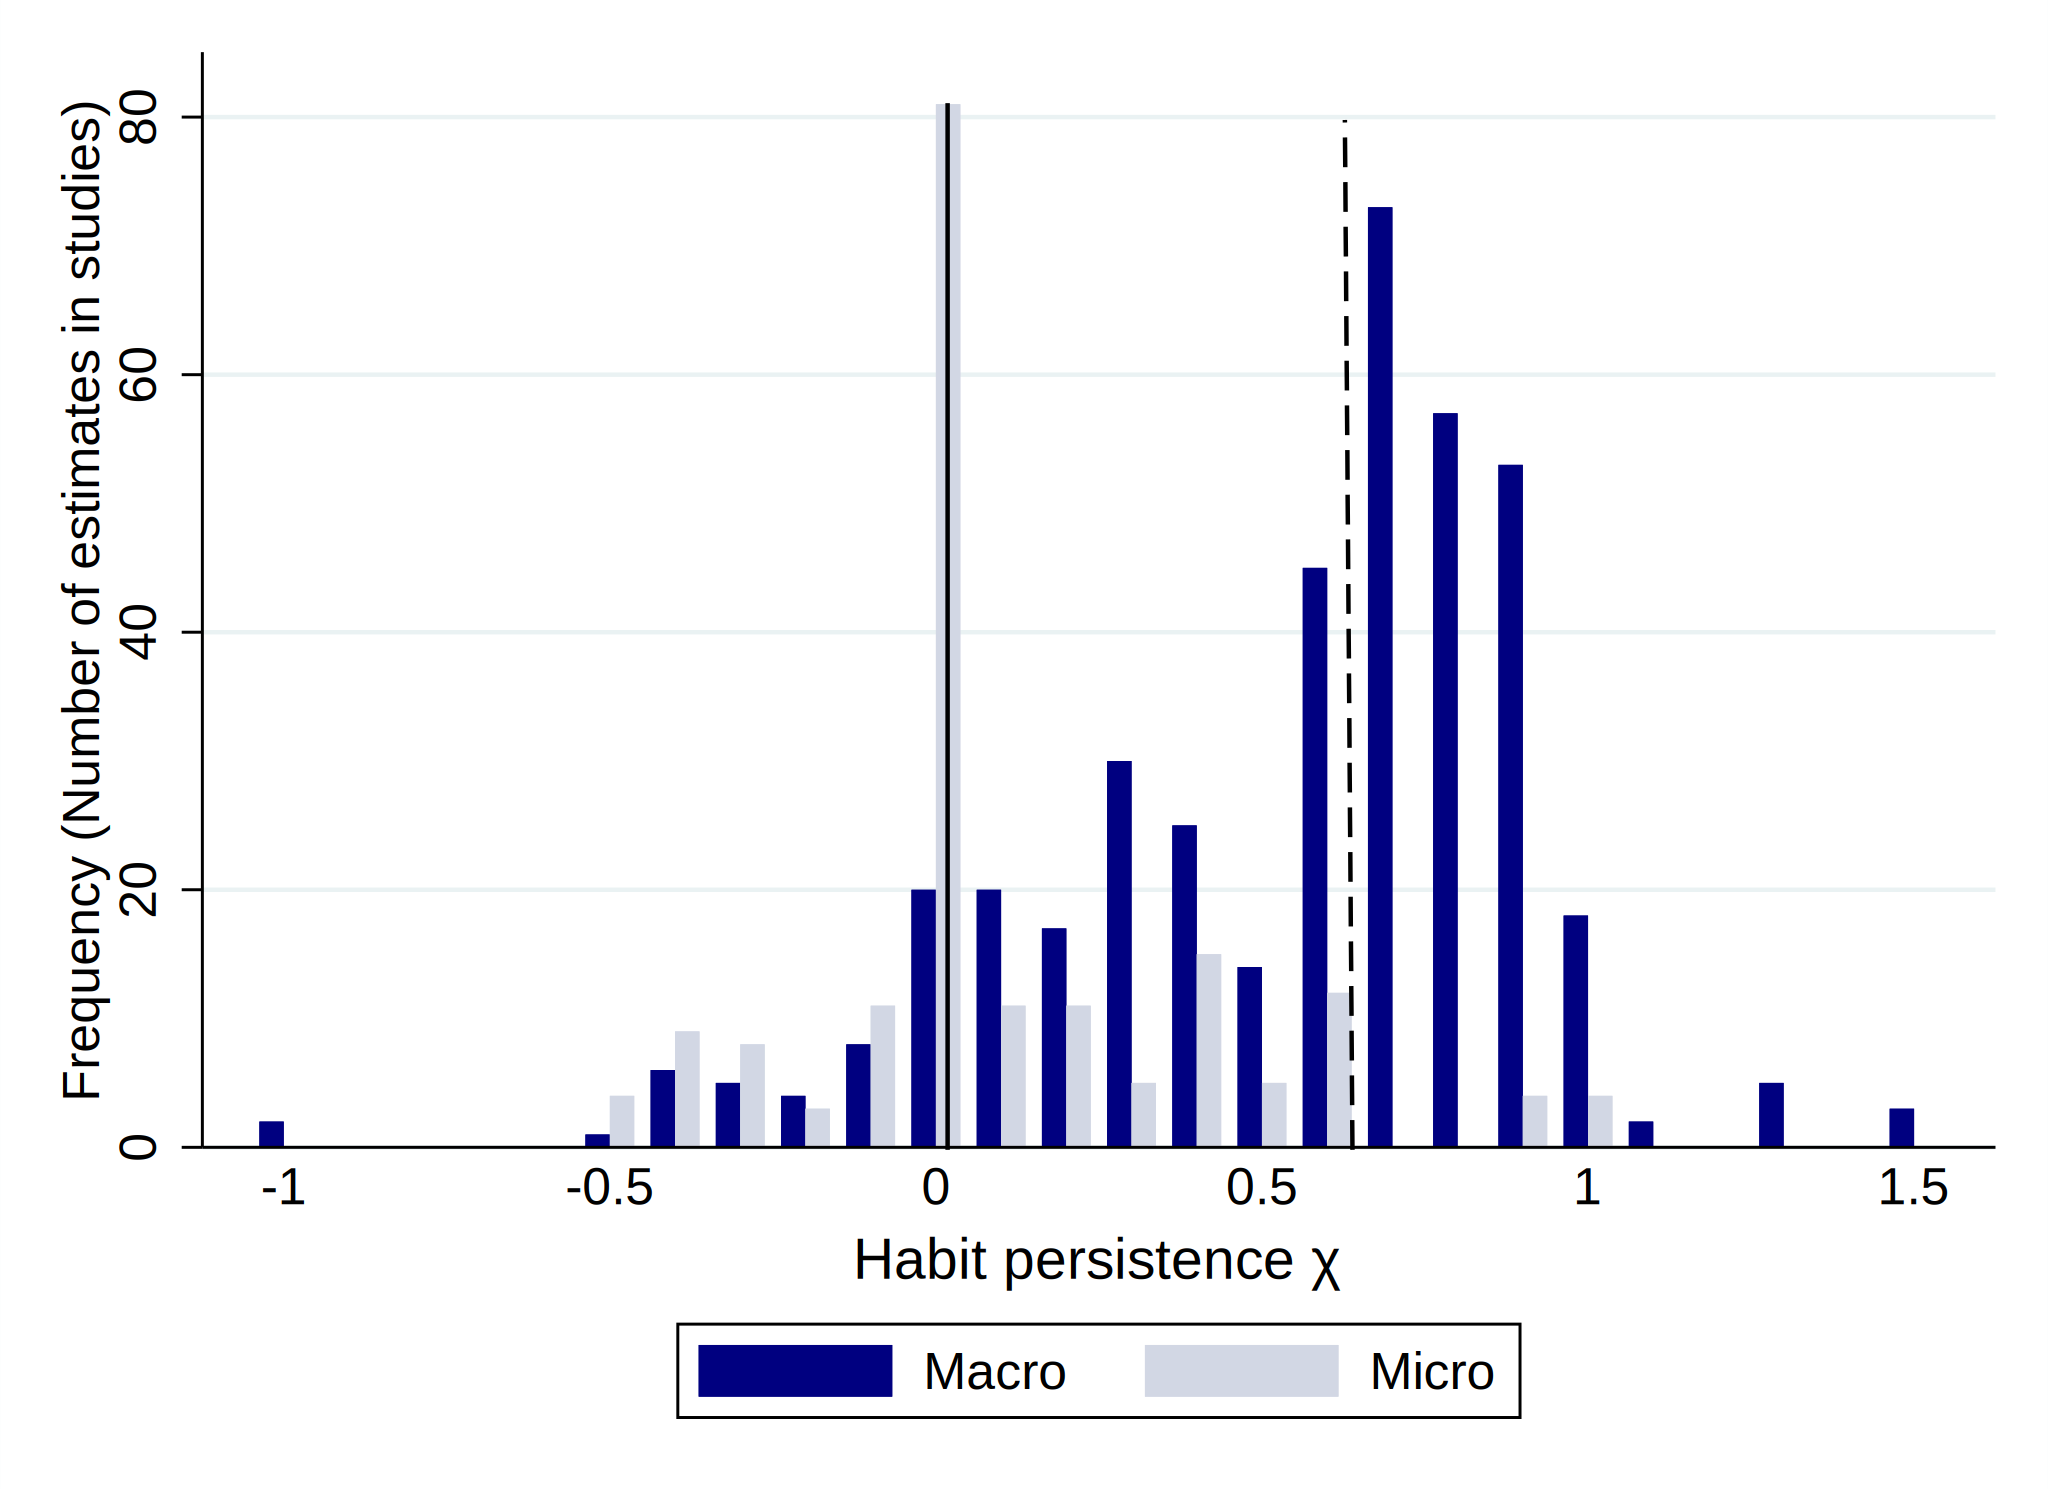
\includegraphics[width=.75\textwidth]{../Figures/microMacroMetaHistogram}
\end{center}
\end{figure}

  \end{itemize}

\end{frame}



\begin{frame}
\frametitle{Claim: It's Not Habits, It's Inattention! (Macro not Micro)}
\jbemph{\large Proposal:\\ Completely drop habits, replace with macro inattention}\\[4mm]
\jbemph{\large Our Setup}
\begin{itemize}
\item   Income Has Idiosyncratic and Aggregate Components
\item   Idiosyncratic Component Is Perfectly Observed
\item   \jbemph{Aggregate Component Is Stochastically Observed}\\
  \begin{itemize}
\item Updating \`a la \cite{calvoPrices}
  \end{itemize}

\end{itemize}
\begin{block}{ Not {\em ad hoc}}
\begin{itemize}
\item Identical: \cite{mrSlumps}, \cite{carroll:epidemicinflQJE}
\item Similar: \cite{reis:inattentive}, \cite{simsInattention},   \dots
% \cite{woodfordImperfect},
\end{itemize}
\end{block}

\end{frame}



\begin{frame}
\frametitle{Why Macro Inattention Is Plausible}

\begin{block}{\textbf{Idiosyncratic Variability Is $\sim$ 100$\times$ Bigger}}
\begin{itemize}
\item  If Same Specification Estimated on Micro vs Macro Data
\item  Pervasive Lesson of All Micro Data
\end{itemize}
\end{block}

\begin{block}{\textbf{Utility Cost of Inattention Small}}
\begin{itemize}
\item  Micro: Critical (and Easy) To Notice You're Unemployed
% \item Unlike \cite{pischkeMicroMacro}
\item  Macro: {\it Not} Critical To Instantly Notice If U $\uparrow$
\end{itemize}
\end{block}
\end{frame}



\begin{frame}
\frametitle{Literature on C Dynamics and Info Frictions}
\small
\begin{itemize}
\item \jemph{C Smoothness:}
\cite{cdSmooth}; \cite{pischkeMicroMacro};
\cite{rotemberg&woodford:macroannual}

\item \jemph{Inattention:}
\cite{mrSlumps}; \cite{reis:inattentive}; \cite{simsInattention}; \cite{mackWiedREStud15}; \cite{gabaixSparsityQJE}; \dots

\item \jemph{Adjustment Costs:} \cite{alvarezGuisoLippi:DurCons}; \cite{chettySzeidl:cCommitmentsEcta}
\item \jemph{Empirical Evidence on Info Frictions:} \cite{coibGor:AER15}; \cite{fuhrerIntrinsicPersistence}; \dots

\item \jemph{Macro Habits:}
\cite{abel:aerhabits}; \cite{constantinidesHabits}; all papers since \cite{cee:habits}

\item \jemph{Micro Habits:}
\cite{dynanHabits}; many recent papers

\end{itemize}

\end{frame}








%\section{\href{http://www.econ2.jhu.edu/people/ccarroll/public/LectureNotes/Consumption/StickyExpectationsC/}{Toy Model}}
%\subsection{Toy Model}
\begin{frame}
\frametitle{Quadratic Utility Frictionless Benchmark}

\begin{block}{\cite{hallRandomWalk} Random Walk}
\phantom{.}
\begin{itemize}
\item \jemph{Total Wealth} (Human$\,+\,$Nonhuman):\\
\begin{center}
{$\wAllLev_{t+1} = (\wAllLev_{t}-\cLevBF_{t})\Rfree+\zeta_{t+1}$}
\end{center}
\item \jemph{C Euler Equation}: \\
\begin{center}
{$\uFunc^{\prime}(\cLevBF_{t}) = \Rfree\beta \Ex_{t}[\uFunc^{\prime}(\cLevBF_{t+1})]$}
\end{center}
\item $\Rightarrow$ \jemph{Random Walk} (for $\Rfree\beta=1$): \\
\begin{center}
{$\Delta \cLevBF_{t+1} = \epsilon_{t+1}$}
\end{center}
\item \jemph{Expected Wealth}: \\
\begin{center}
{$\wAllLev_{t} = \Ex_{t}[\wAllLev_{t+1}] = \Ex_{t}[\wAllLev_{t+2}] = \dots$}
\end{center}
\end{itemize}
\end{block}

\end{frame}


\begin{frame}
\frametitle{Sticky Expectations---Individual $\mathbf{c}$}

\begin{itemize}
\item
Consumer who happens to update at $t$ and $t+n$
\begin{eqnarray*}
\ifnumSw         \cLevBF_{t  } & = & (\rfree/\Rfree)\wAllLev_{t} \label{eq:ct}
\ifnumSw \\      \cLevBF_{t+1} & = & (\rfree/\Rfree)\perc{\wAllLev}_{t+1} = (\rfree/\Rfree)     \wAllLev _{t} = \cLevBF_{t}
%\ifnumSw \\      \cLevBF_{t+2} & = & (\rfree/\Rfree)\perc{\wAllLev}_{t+2} = (\rfree/\Rfree)     \wAllLev _{t} = \cLevBF_{t}
\ifnumSw \\               \vdots  &  & \vdots \nonumber
\ifnumSw \\        \cLevBF_{t+n-1} & = & \cLevBF_{t}
\label{eq:ctpn}
\end{eqnarray*}

\item
Implies that $\Delta^{n} \wAllLev_{t+n} \equiv \wAllLev_{t+n}-\wAllLev_{t}$ is white noise

\item So \jbemph{individual} $\mathbf{c}$ is RW across updating periods:
\begin{eqnarray*}
\ifnumSw  \mathbf{c}_{t+n}-\mathbf{c}_{t} & = & (\rfree/\Rfree)\underbrace{(\wAllLev_{t+n}-\wAllLev_{t}) }_{\Delta^{n} \wAllLev_{t+n}}
\end{eqnarray*}
%\item \jbemph{No persistence in individual c growth}
\end{itemize}
\end{frame}

\begin{frame}
\frametitle{Sticky Expectations---Aggregate $\mathbf{C}$}

\begin{itemize}
\setlength{\itemsep}{2mm}
\item Pop normed to one, uniformly dist on $[0,1]$:
$\CLevBF_{t} = \int_{0}^{1} \cLevBF_{t,i}\,\text{d}i$

\item \jbemph{\cite{calvoPrices}-Type Updating of Expectations:}
\begin{itemize}
\item Probability $\Pi = 0.25$ (per quarter)
%\item NOT Muth/Lucas/Pischke/Reis signal extraction
\end{itemize}

\item Economy composed of many sticky-$\Ex$ consumers:
\begin{eqnarray*}
 \CLevBF_{t+1} & = & (1-\Pi) \underbrace{\CLevBF^{\cancel{{\pi}}}_{t+1}}_{=\CLevBF_{t}} \label{eq:Ctp1} + \Pi \CLevBF^{{\pi}}_{t+1}
 \\
%\end{eqnarray*}
%\begin{eqnarray*}
  \Delta \mathbf{C}_{t+1} & \approx & \underbrace{(1-\Pi)}_{{}\equiv\chi=0.75} \Delta \mathbf{C}_{t} + \epsilon_{t+1}
\end{eqnarray*}
\item \jbemph{Substantial persistence ($\chi=0.75$) in aggregate C growth}
\end{itemize}
\end{frame}


\begin{frame}
\frametitle{One More Ingredient \dots}

\begin{itemize}
\setlength{\itemsep}{3mm}
\item  \jbemph{Differences: Idiosyncratic vs Aggregate shocks}

\begin{itemize}
\setlength{\itemsep}{2mm}
\item  \jemph{Idiosyncratic shocks:} Frictionless observation
  \begin{itemize}
  \setlength{\itemsep}{1mm}
  \item I notice if I am fired, promoted, somebody steals my wallet
  \item  True RW with respect to these
  \end{itemize}
\item \jemph{Aggregate shocks:} Sticky observation
 \begin{itemize}
   \setlength{\itemsep}{1mm}
  \item May not instantly notice changes in aggregate productivity
  \end{itemize}
\end{itemize}

\item \jbemph{Result:}
\begin{itemize}
  \setlength{\itemsep}{1mm}
\item  \jemph{Idiosyncratic $\Delta \mathbf{c}$}: dominated by frictionless RW part
\item  \jemph{Aggregate     $\Delta \mathbf{C}$}: highly serially correlated\\
  Law of large numbers $\Rightarrow$ idiosyncratic part vanishes
\end{itemize}
\end{itemize}

\end{frame}



%\section{The Real Model}
%\subsection{Frictionless Setup}
\begin{frame}
\frametitle{Serious Models}

\begin{block}{Partial Equilibrium/Small Open Economy}
\begin{itemize}
\item  CRRA Utility
\item  Idiosyncratic Shocks Calibrated From Micro Data
\item  Aggregate Shocks Calibrated From Macro Data
\item Markov Process (Discrete RW) for Aggr Income Growth
  \begin{itemize}
  \item Handles changing growth `eras'
  \end{itemize}
\item  Liquidity Constraint
\item  Mildly Impatient Consumers
\end{itemize}
\end{block}

\begin{block}{DSGE Heterogeneous Agents (HA) Model}
\begin{itemize}
\item  Same!
\end{itemize}
\end{block}
\end{frame}


\begin{frame}
\frametitle{Solving the Models}

All results are generated using the open-source Econ-ARK toolkit:\\
\texttt{github.com/Econ-ARK/HARK/cAndCwithStickyE}

%\footnotesize
%\begin{tabular}{ll}
%\texttt{github.com/Econ-ARK} & All project resources
%\\ \texttt{github.com/Econ-ARK/HARK} & The HA toolkit
%\\ \texttt{github.com/Econ-ARK/HARK/cAndCwithStickyE} & Results from this paper
%\\ \texttt{github.com/Econ-ARK/PARK} & Presentations about toolkit
%\\ \texttt{github.com/Econ-ARK/PARK/SciPy2018.pdf} & Overview paper
%\\ 
%\end{tabular} \normalsize
%\bi
%\item \url{github.com/econ-ark/hark}, in  `cAndCwithStickyE` 
%\ei

\vspace*{0.3cm}
For a portal to the Econ-ARK project, go to: 
\bi
\item \url{http://econ-ark.org}
\ei

\vspace*{0.3cm}
More Econ-ARK/HARK in next session ``Econ-Developers Summit'' at 11:10 in room G.012 Pio XII

\end{frame}



\begin{frame}
\frametitle{Income Process}

\begin{itemize}
\item  Individual's labor productivity is
$$
\pmb{\ell}_{t,i} = \overbrace{\theta_{t,i}\Theta_{t}}^{\equiv\,\pmb{\theta}_{t,i}}\overbrace{{p}_{t,i} {P}_{t}}^{\equiv\, \pLev_{t,i}}
$$

\item  Idiosyncratic and aggregate $p$ evolve according to
\begin{eqnarray*}
{{p}}_{t+1,i} & =&  \phantom{\jemph{\PtyGro}_{t+1}}{{p}}_{t,i} \psi_{t+1,i}  \\
 {P}_{t+1\phantom{,i}} & =&  \jemph{\PtyGro}_{t+1} {P}_{t\phantom{,i}}\Psi_{t+1}
\end{eqnarray*}

%\item  $\Ex_{t}[\theta_{t+n}]=\Ex_{t}[\Theta_{t+n}]=\Ex_{t}[\pShk_{t+n}]=\Ex_{t}[\PShk_{t+n}]=1\quad\forall~n>0$

  \item \jbemph{$\PtyGro$ is Markov `underlying' aggregate pty growth}
    \begin{itemize}
    \setlength{\itemsep}{1mm}
    \item Discrete (bounded) random walk
    \item Calibrated to match postwar US pty growth variation
    \item Generates predictability in income growth (for IV regressions)
    \end{itemize}
  \end{itemize}
\end{frame}

\begin{frame}
\frametitle{\cite{blanchardFinite} Mortality and Insurance}

\begin{itemize}
\item  Household survives from $t$ to $t+1$ with probability $(1-\PDies)$:
\begin{equation*} \ifnumSw
{p}_{t+1,i} =
  \begin{cases}
    1 & \text{for newborns}
\\ \ifnumSw  {p}_{t,i} \psi_{t+1,i} & \text{for survivors}
  \end{cases}
\end{equation*}


\item Blanchardian scheme:
\begin{equation*} \ifnumSw
\kLevBF_{t+1,i}  =
\begin{cases}
                         0                       & \text{if HH $i$ dies, is replaced by newborn}
\\ \aLevBF_{t,i} \big/(1-\PDies) & \text{if household $i$ survives}
\end{cases} \label{eq:tontine}
\end{equation*}
\item Implies for aggregate:
\begin{eqnarray*}
\ifnumSw      \KLevBF_{t+1} & = & \int_{0}^{1} \left(\frac{1-\pDies_{t+1,i}}{1-\PDies}\right) \aLevBF_{t,i}   \,\text{d}i   \label{eq:Ktp1} = \ALevBF_{t}
\ifnumSw  \\          K _{t+1} & = &  \ALev_{t}\big/(\Psi_{t+1} \PtyGro_{t+1}) \ifnumSw
\end{eqnarray*}


%\item Implies steady-state distribution of ${p}$ with variance:
%
%\begin{eqnarray}
% \text{var}(p) & = & \left(\frac{\PDies}{1-(1-\PDies) \Ex[\pShk^{2}]}-1\right) \nonumber
%\end{eqnarray}

\end{itemize}
\end{frame}



\begin{frame}
\frametitle{Resources}

\begin{itemize}
\item  Market resources:
%labor income+capital+capital income:
$$\mLevBF_{t,i} = \underbrace{{\bf \Wage_t} \pmb{\ell}_{t,i}}_{\equiv\, \yLevBF_{t}} + \underbrace{{\Rprod_t}}_{\daleth\,+\,\rfree_t} \kLevBF_{t,i}$$
\item End-of-Period `Assets'---Unspent resources:
\begin{eqnarray*}
\ifnumSw \mathbf{a}_{t,i} & = & \mathbf{m}_{t,i}-\mathbf{c}_{t,i}
\end{eqnarray*}

\item Capital transition depends on prob of survival $1-\PDies$:
\begin{eqnarray*}
\ifnumSw  \mathbf{k}_{t+1,i} & = &   \mathbf{a}_{t,i}\big/(1-\PDies)
\end{eqnarray*}

\end{itemize}

\end{frame}



\begin{frame}
\frametitle{Frictionless Solution}

\begin{itemize}
\setlength{\itemsep}{2mm}
\item  For exposition: Assume constant $\Wage$ and $\Rprod$
\item  Normalize everything by $\pLev_{t,i}\equiv{p}_{t,i} {P}_{t}$, e.g.\ $m_{t,i}=\mathbf{m}_{t,i}\big/({p}_{t,i}{P}_{t})$
\item $\cFunc(m,\PtyGro)$ is the function that solves:
\begin{equation*}
 v(m_{t,i},\Phi_t) = \max_{\cRat} \util(\cRat) + \PLives\DiscFac \Ex_{t}\big[(\Phi_{t+1}\pmb{\pShk}_{t+1,i})^{1-\CRRA}v(m_{t+1,i},\Phi_{t+1})\big]
\end{equation*}

\item Level of consumption:
$$\cLevBF_{t,i} = \cFunc(m_{t,i}, \PtyGro_t) \times {p}_{t,i}{P}_{t}$$

%\item Test: $\eta=\chi=\alpha=0$ in
%\input \eq/microEuler.tex
\end{itemize}
\end{frame}

%\subsection{Sticky Expectations}
\begin{frame}
\frametitle{Sticky Expectations about Aggregate Income}

\jbemph{\large Calvo Updating of Perceptions of Aggregate Shocks}\\
\bi
\item {\it True} Permanent income: ${P}_{t+1} =  \PtyGro_{t+1} {P}_{t}\Psi_{t+1}$\\
\item Tilde ($\perc{P}$) denotes perceived variables
\item \jemph{Perception for consumer who has not updated for $n$ periods:}
$$
  \perc{P}_{t,i}=\Ex_{t-n}\big[P_t\big\vert\Omega_{t-n}\big]=\Phi_{t-n}^nP_{t-n}
$$
because $\Phi$ is random walk
\ei
\end{frame}



\begin{frame}
\frametitle{Sticky Expectations about Aggregate Income}

\jbemph{\large Sequence Within Period}\\
\begin{enumerate}
\setlength{\itemsep}{2mm}
\item Income shocks are realized and every individual sees her true $\mathbf{y}$ and $\mathbf{m}$,
i.e.\ $\mathbf{y}_{t,i}=\perc{\mathbf{y}}_{t,i}$ and $\mathbf{m}_{t,i}=\perc{\mathbf{m}}_{t,i}$ for all $t$ and $i$

\item Updating shocks realized: $i$ observes true $P_t, \PtyGro_t$ w/ prob $\Pi$;\\
forms perceptions of her normalized market resources $\perc{\mLev}_{t,i}$

\item Consumes based on her perception, \jemph{using $\cFunc(\perc{m}_{t,i},\perc{\PtyGro}_{t,i})$}\\[1mm]

  \jemph{\textbf{Key Assumption:}}\\
    \begin{itemize}
    \item  People act as if their perceptions about aggregate state $\{\perc{P}_{t,i},\perc{\PtyGro}_{t,i}\}$
are the true aggregate state $\{P_t,\PtyGro_t\}$
    \end{itemize}

\end{enumerate}

\end{frame}


\begin{frame}
\frametitle{Behavior under Sticky Expectations}
\bi
\setlength{\itemsep}{2mm}
\item \jemph{Normalized resources:}
  \begin{itemize}
  \item   $\jemph{m_{t,i}}\equiv\mathbf{m}_{t,i}\big/({p}_{t,i}{P}_{t})$ is {\it actual}\\
\item \jemph{\phantom{Normalized resources:}} $\jemph{\perc{m}_{t,i}}\equiv\mathbf{m}_{t,i}\big/({p}_{t,i}\perc{P}_{t,i})$ is {\it perceived}
  \end{itemize}

\item \jbemph{Usually $\perc{m}_{t,i}\not={m}_{t,i}$ because $P_{t}$ not perfectly observed}\\
  \begin{itemize}
  \item in levels: $\perc{\mathbf{m}}_{t,i}=\mathbf{m}_{t,i}$; but normalized: $\perc{m}_{t,i}\not={m}_{t,i}$
  \end{itemize}

\item {\small Consumers behave according to frictionless consumption function}

\item But \jbemph{based on $\perc{m}_{t,i}$} (not ${m}_{t,i}$):
\begin{eqnarray*}
 \perc{c}_{t,i} & = & \cFunc(\perc{m}_{t,i},\perc{\PtyGro}_{t,i}) \\
 \cLevBF_{t,i} & = & \perc{c}_{t,i}\times{p}_{t,i}\perc{P}_{t,i}
\end{eqnarray*}

\item Correctly perceive level of their own spending $\cLevBF_{t,i}$
\end{itemize}
%\input \eq/aBari.tex

%\input \eq/kBartp1i.tex
\end{frame}





%%%%%%%%%%%%%%%%%%%%%%%%%%%%%%%%%%%%%%%%%%%%%%%%%%%%%%%%%%%%%%%%%%%%%%%%%%%%%%%%%%%%%%%%%%%%%%%%%%%%%%%%%%%%%%%%%%%%%%%%%%%%%%%%%%%%%

%\subsection{`Representative Agent' Version}
\begin{frame}
\frametitle{DSGE Heterogeneous Agents Model}

\begin{itemize}
\item  Idiosyncratic and aggregate shocks same as PE/SOE
\item  Endogenous $\Wage_t$ and $\Rprod_t$
\item Aggregate market resources $M_t$ is a state variable
\small
\begin{equation*}
 v(m_{t,i},\jemph{M_t},\PtyGro_t) = \max_{\cRat} \util(\cRat) + \PLives\DiscFac \Ex_{t}\big[(\Phi_{t+1}\pmb{\pShk}_{t+1,i})^{1-\CRRA}v(m_{t+1,i},\jemph{M_{t+1}},\PtyGro_{t+1})\big]
\end{equation*}
\normalsize
\item Solved using \cite{ksHetero}
\item  Perception dynamics identical to sticky PE/SOE:
$$\cLevBF_{t,i} = \cFunc(\perc{m}_{t,i},\jemph{\perc{M}_{t,i}},\perc{\PtyGro}_{t,i})\times{p}_{t,i}\perc{P}_{t,i}$$
\end{itemize}
\end{frame}



\begin{frame}
\frametitle{Regressions on Simulated and Actual Data}
\jbemph{\cite{dynanHabits}/\cite{som07} Specification:}
$$
 \Delta \log \mathbf{C}_{t+1} \approx  \varsigma +\chi \Ex[ \Delta \log \mathbf{C}_{t}] + \eta \Ex[\Delta \log \mathbf{Y}_{t+1}]+\alpha A_{t}   +\epsilon_{t+1}
$$
\vspace*{-0.5cm}
\begin{itemize}
\setlength{\itemsep}{2mm}
\item \jbemph{$\chi$: Extent of habits}\\
\jemph{Data: Micro:} $\chi^{\text{Micro}} = 0.1$ (EER 2017 paper)\\
\hspace*{1.1cm}\jemph{Macro:} $\chi^{\text{Macro}} = 0.6$

\item  \jbemph{$\eta$: Fraction of Y going to `rule-of-thumb' C\,=\,Y types}\\
\jemph{Data: Micro:} $0<\eta^{\text{Micro}} <1$ (Depends \dots)\\
\hspace*{1.1cm}\jemph{Macro:} $\eta^{\text{Macro}} \approx 0.5$ (\cite{cmModel})

\item  \jbemph{$\alpha$: Precautionary saving (micro) or IES (Macro)}\\
\jemph{Data: Micro:} $\alpha^{\text{Micro}}<0$ (\cite{zeldes:jpe})\\
\hspace*{1.1cm}\jemph{Macro:} $\alpha^{\text{Macro}}<0$ (but small)\\
{[In GE $\rfree$ depends roughly linearly on $A$]}
\end{itemize}

\end{frame}



\begin{frame}
\frametitle{Micro vs Macro: Theory and Empirics}
\begin{eqnarray}
\ifnumSw\Delta \log \mathbf{C}_{t+1} & \approx & \varsigma+\chi \Delta \log \mathbf{C}_{t}+\eta \Ex_{t}[\Delta \log \mathbf{Y}_{t+1}]+\alpha A_{t}+\epsilon_{t+1} \nonumber
\end{eqnarray}

\begin{center}
\begin{tabular}{llccc}
\toprule
        &        & $\chi$       & $\eta$          & $\alpha$
\\ \midrule \multicolumn{2}{l}{Micro (Separable)}
\\    & Theory                 & $\approx 0  $      & $0 < \eta < 1 $ & $< 0$
\\        & Data                   & $\approx 0  $      & $0 < \eta < 1 $ & $< 0$
\\ \midrule \multicolumn{2}{l}{Macro}
\\ & Theory: Separable          & $\approx 0   $     & $\approx 0$           & $< 0$
\\ & Theory: CampMan            & $\approx 0   $     & $\approx 0.5$           & $< 0$
\\ & Theory: Habits             & $\approx 0.75$     & $\approx 0$           & $< 0$
\\ \bottomrule
%\\ & Data:CampMan            &                    & $0.50$                  & $> 0$
%\\ & Data (Sommer)           & $0.7$              & $0.15$                  & $> 0$
%\\ Habits  & $\approx 0.75 $    & $\approx 0$           & $ > 0        $
\end{tabular}
\end{center}
\end{frame}





\begin{frame}
\frametitle{Calibration I}
%\ptsize{9}
\small
\input ../Tables/Calibration_1.tex


\end{frame}


\begin{frame}
\frametitle{Calibration II}
%\ptsize{9}
\small
\input ../Tables/Calibration_2.tex


\end{frame}



%\subsection{Simulated Data}
\begin{frame}
\frametitle{Micro Regressions: Frictionless}
\input \eq/CGrowCross.tex
%\ptsize{10}
\small
\begin{eqnarray}
\ifnumSw\CGrowCross    \label{eq:CGrowCross}     \nonumber
\end{eqnarray}

\input ../Tables/CGrowCross_SlidesF.tex
\normalsize

\end{frame}

\begin{frame}
\frametitle{Micro Regressions: Sticky}
\input \eq/CGrowCross.tex
%\ptsize{10}
\small
\begin{eqnarray}
\ifnumSw\CGrowCross    \label{eq:CGrowCross}     \nonumber
\end{eqnarray}

\input ../Tables/CGrowCross_SlidesS.tex
\normalsize
\end{frame}


%\subsection{Actual U.S. Data}
\begin{frame}
\frametitle{Empirical Results for U.S.}

%\providecommand{\DirCampManVsStickyE}{/Volumes/Data/Work/cAndCwithStickyEArchive/Empirical/US/Results/LaTeX/tables}

\scriptsize

%\input \TabsDir/slides/tEmpiricalConsNondurables.tex
\input ../Tables/tEmpiricalCons.tex
\normalsize
\end{frame}



\begin{frame}
\frametitle{Small Open Economy: Sticky}

\scriptsize
%\begin{center}
\input ../Tables/SOEmrkvSimRegS.tex

\end{frame}



\begin{frame}
\frametitle{Small Open Economy: Frictionless}

\scriptsize
%\begin{center}
\input ../Tables/SOEmrkvSimRegF.tex

\end{frame}



\begin{frame}
\frametitle{Heterogeneous Agents DSGE: Sticky}

\scriptsize
%\begin{center}
\input ../Tables/DSGEmrkvSimRegS.tex

\end{frame}



\begin{frame}
\frametitle{Heterogeneous Agents DSGE: Frictionless}

\scriptsize
%\begin{center}
\input ../Tables/DSGEmrkvSimRegF.tex

\end{frame}




%\section{Conclusion}
%\subsection{Conclusion}


\begin{frame}
\frametitle{Utility Costs of Stickiness}

\begin{itemize}
\item  Simulate expected lifetime utility when market resources nonstochastically equal to $\Wage_t$ at birth under \jbemph{frictionless}
\begin{equation*}
\overline{\vFunc}_0 \equiv \Ex [ \vFunc(\Wage_t,\cdot)]
\end{equation*}
and \jbemph{sticky expectations}:
$ \displaystyle
\overline{\widetilde{\vFunc}}_0 \equiv \Ex [ \widetilde{\vFunc}(\Wage_t,\cdot)]
$
\item Expectations taken over state variables other than $\mLev_{t,i}$
\item Newborn's
willingness to pay (as fraction of permanent income) to avoid having
sticky expectations:
\begin{eqnarray*}\label{eq:WTP}
\omega & = & 1 - \left( \frac{\overline{\widetilde{\vFunc}}_0}{\overline{\vFunc}_0} \right)^{\frac{1}{1-\CRRA}}
\end{eqnarray*}
\item \jbemph{$\omega \approx 0.05\%$ of permanent income}\\
$\omega_{SOE}=4.82\text{e--4}$; $\omega_{HA-DSGE}=4.51\text{e--4}$
\end{itemize}
\end{frame}




\begin{frame}
\frametitle{Conclusion}
\jbemph{
Model with `Sticky Expectations' of aggregate variables can match both micro and macro consumption dynamics}

\begin{eqnarray}
\ifnumSw\Delta \log \mathbf{C}_{t+1} & \approx & \varsigma+\chi \Delta \log \mathbf{C}_{t}+\eta \Ex_{t}[\Delta \log \mathbf{Y}_{t+1}]+\alpha A_{t}+\epsilon_{t+1} \nonumber
\end{eqnarray}

\begin{center}
\begin{tabular}{llccc}
\toprule
        &        & $\chi$       & $\eta$          & $\alpha$
\\ \midrule \multicolumn{2}{l}{Micro }

\\        & Data                   & $\approx 0  $      & $0 < \eta < 1 $ & $< 0$
\\    & Theory: Habits                &  $\approx 0.75$       & $0 < \eta < 1 $ & $< 0$
\\        & Theory: Sticky Expectations                  & $\approx 0  $      & $0 < \eta < 1 $ & $< 0$
\\ \midrule \multicolumn{2}{l}{Macro}
\\ & Data             & $\approx 0.75$     & $\approx 0$           & $< 0$
\\ & Theory: Habits             & $\approx 0.75$     & $\approx 0$           & $< 0$
\\ & Theory: Habits             & $\approx 0.75$     & $\approx 0$           & $< 0$
\\ \bottomrule
%\\ & Data:CampMan            &                    & $0.50$                  & $> 0$
%\\ & Data (Sommer)           & $0.7$              & $0.15$                  & $> 0$
%\\ Habits  & $\approx 0.75 $    & $\approx 0$           & $ > 0        $
\end{tabular}
\end{center}

\end{frame}

%%%%%%%%%%%%%%%  bibliography
%%%%%%%%%%%%%%%%%%%%%%%%%%%%%%%%%%%%%%%%%%%%%%%%%%%%%%%%%%%%%%%%%%%%%%%%%%%%%%%%%%%%%%%%%%%%%%%%%%%%%%%%%%%%%%
\tiny

\beamerdefaultoverlayspecification{<*>}

\begin{frame}[t,allowframebreaks]
\frametitle{References}

%\input econtexBibMake

%\write18{if [ `kpsewhich economics.bib` != '' ]; then touch economics.bib    ; fi} # This should be done only for final versions AFTER bibexport has occurred and \jobname.bib is populated
%\write18{if [ ! -f \jobname.bib     ]; then touch \jobname.bib     ; fi}
%\write18{if [ ! -f \jobname-Add.bib ]; then touch \jobname-Add.bib ; fi}

\bibliographystyle{econtex}
\bibliography{economics,cAndCwithStickyE-Slides,cAndCwithStickyE-Slides-Add}


\end{frame}

\normalsize



\begin{frame}
  \frametitle{Markov Process for Aggregate Productivity Growth $\Phi$}

$
\pmb{\ell}_{t,i} = \theta_{t,i}\Theta p_{t,i} {P}_{t},\quad
p_{t+1,i} =  {{p}}_{t,i} \psi_{t+1,i},  \quad
 {P}_{t+1} =  \PtyGro_{t+1} {P}_{t}\Psi_{t+1}
$
\bi
\item $\Phi_t$ follows bounded (discrete) RW
\item 11 states; average persistence 2 quarters
\item Flexible way to match actual pty growth data
\ei
  \begin{figure}
\begin{center}
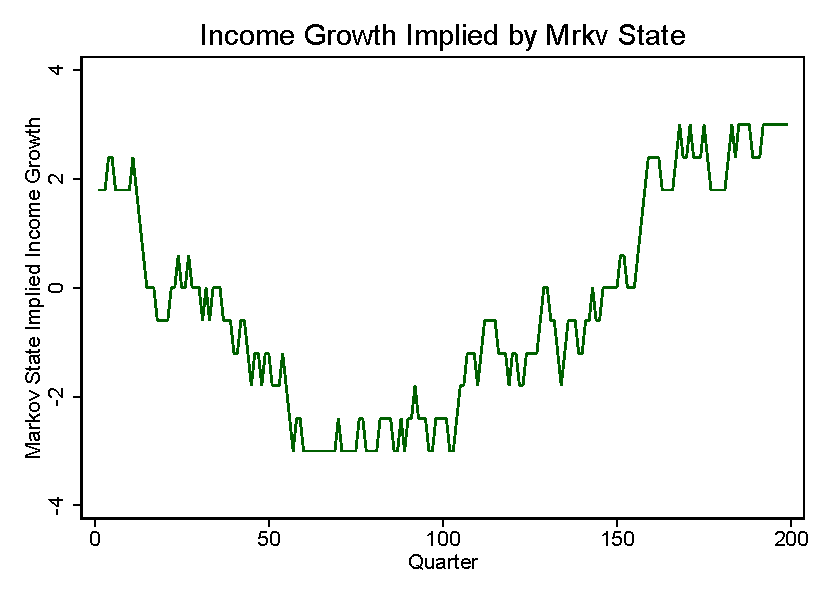
\includegraphics[width=.75\textwidth]{../Figures/MrkvStateGrowth}
\end{center}
\end{figure}

\end{frame}



\begin{frame}
\frametitle{Equilibrium}

\footnotesize
\input ../Tables/EqbmSlides.tex

\end{frame}


\begin{frame}
\frametitle{Cost of Stickiness}
Define (for given parameter values):
\begin{center}
\begin{tabular}{rl}
${v}(\Wage_t,\cdot)$ & Newborns' expected value for frictionless model
\\ $\grave{v}(\Wage,\cdot)$ & Newborns' expected value if $\sigma^{2}_{\psi}=0$
\\ $\perc{v}(\Wage,\cdot)$ & Newborns' expected value from sticky behavior
\end{tabular}
\end{center}

Fact suggested by theory (and confirmed numerically):
\input \eq/vApprox.tex

Guess (and verify) that:
\input \eq/vApproxSticky.tex


\end{frame}


\begin{frame}
\frametitle{Cost of Stickiness: $\omega$ and $\Pi$}

Costs of stickiness $\omega$ and prob of aggr info updating $\Pi$

\begin{figure}
\label{costOfStickiness}
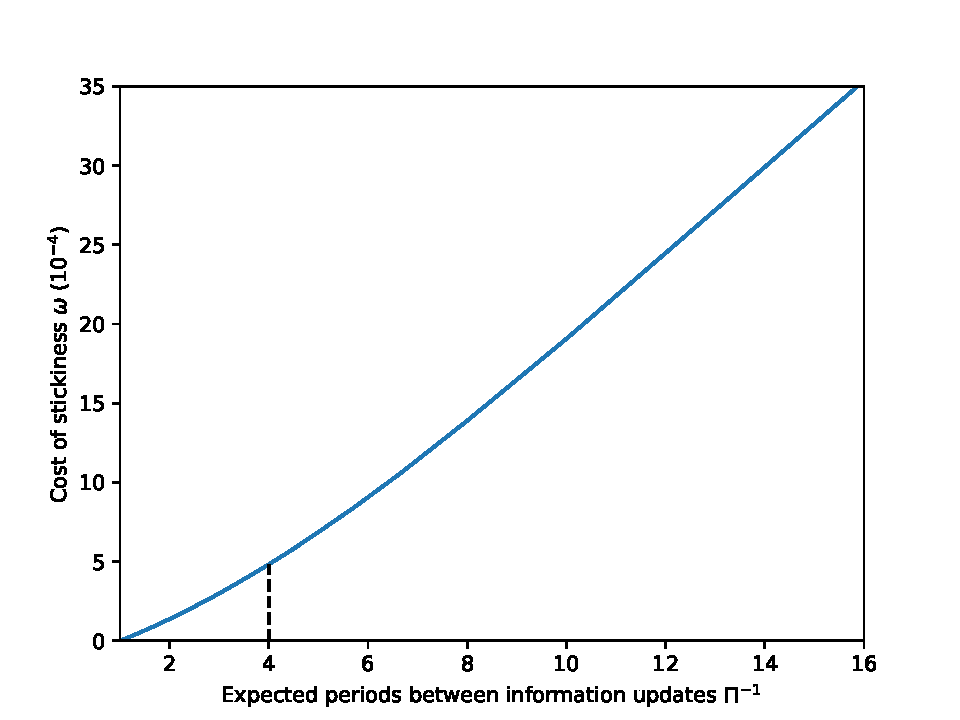
\includegraphics[width=0.9\textwidth, height=6cm]{../Figures/uCostvsPiInv.pdf}\\
\tiny Notes: The figure shows how the utility costs of updating $\omega$ depend on the probability of updating of aggregate information $\Pi$ in the SOE model.
\end{figure}

\end{frame}




\begin{frame}
\frametitle{Cost of Stickiness: Solution}
Suppose utility cost of attention is $\iota\Pi$.
\begin{itemize}
\item If Newborns Pick Optimal $\Pi$, they solve
\end{itemize}

\input \eq/pickPi.tex

Solution:
\input \eq/bestPi.tex

Optimal $\Pi$ characteristics:
\begin{itemize}
\item Increasing in $\kappa$ (`importance' to value of perm shocks)
\item Increasing in $\sigma_{\psi}$ (`magnitude' of perm shocks)
\item Decreasing as attention becomes more costly: $\iota \uparrow$
\end{itemize}


\end{frame}


\begin{frame}
\frametitle{Is Muth--Lucas--Pischke Kalman Filter Equivalent?}

\jbemph{No.}\\
\cite{muthOptimal}--\cite{lucas:imperfectInfo}--\cite{pischkeMicroMacro} Kalman filter
\begin{itemize}
\item  All you can see is Y
\begin{itemize}
\item Lucas: Can't distinguish agg. from idio.
\item Muth--Pischke: Can't distinguish tran from perm
\end{itemize}

\item Here: Can see own circumstances perfectly

\item Only the (tiny) aggregate part is hard to see

\item \jbemph{Signal extraction for aggregate $\mathbf{Y}_t$ gives too little persistence in $\Delta \mathbf{C}_t$: $\chi\approx 0.17$}


\end{itemize}

\end{frame}


\begin{frame}
\frametitle{Muth--Pischke Perception Dynamics}


\begin{itemize}
\item Optimal signal extraction problem (Kalman filter):\\
Observe $\mathbf{Y}$ (aggregate income), estimate $P$, $\Theta$
\item Optimal estimate of ${P}$:
\begin{eqnarray*}
   \ifnumSw  \hat{{P}}_{t+1} & = & \Pi \mathbf{Y}_{t+1} + (1-\Pi) \hat{{P}}_{t},
\end{eqnarray*}
where for signal-to-noise ratio $\varphi = \sigma_{\PShk}/\sigma_{\Theta}$:
\input \eq/SigToNoise.tex
\item But if we calibrate $\varphi$ using observed macro data
  \begin{itemize}

\item \jbemph{$\Rightarrow \Delta \log \mathbf{C}_{t+1} \approx $ 0.17 $ \Delta \log \mathbf{C}_{t}$}
\item \jbemph{Too little persistence!
}
\end{itemize}
\end{itemize}

\end{frame}






\end{document}
